\documentclass[a4paper,UTF8]{article}
\usepackage{ctex}
\usepackage[margin=1.25in]{geometry}
\usepackage{color}
\usepackage{graphicx}
\usepackage{amssymb}
\usepackage{amsmath}
\usepackage{amsthm}
%\usepackage[thmmarks, amsmath, thref]{ntheorem}
\theoremstyle{definition}
\newtheorem*{solution}{Solution}
\newtheorem*{prove}{Proof}
\usepackage{multirow}
\usepackage{url}
\usepackage{enumerate}
\usepackage{listings}
\usepackage{caption}
\usepackage{subfigure}
\usepackage[colorlinks,linkcolor=black, anchorcolor=black,citecolor=black,]{hyperref}


\begin{document}
\title{\textbf{《计算机图形学》九月报告}}
\author{学号:181860077 姓名:佘帅杰,\href{mailto:3121416933@qq.com}{3121416933@qq.com}}
\maketitle

\section{综述}
\begin{enumerate}
    \item 阅读框架代码,初步对代码结构有所了解,同时对pyQt5也有一定的了解
    
    \item 实现直线绘制算法DDA,Bresenham,同时加上功能调用使得GUI和Cli能够
    正常的使用直线绘制算法
    
    \item 实现了利用中点圆绘制算法绘制椭圆和多边形,并在Cli中功能调用,正常使用

    \item 添加算法正确性检查框架,使用多种方法对绘图正确性进行检查
    
    \item 基于GUI框架实现鼠标选中图元
\end{enumerate}


\section{算法介绍}
\subsection{框架代码分析}
在实现之前自然要对拿到手的框架代码进行阅读和分析,可以显然的看到代码
主要都分布在三个文件中,分别进行阅读和分析
\subsubsection{cg\_algorithm.py}
这个文件主要就是实现绘图代码的算法,每一个函数基本都代表这一个需要
实现的功能或者是算法,每一个函数接受绘图所必须的点,一般都是以列表的
形式给出,其他的参数一般就是一些可选参数(如:想要实现的后台算法种类)
这一块结构比较简单,也是实现的核心和重点
\subsubsection{cg\_cli.py}
cli文件主要是负责解析命令行文件,并做出回应。基本的功能就是按行读取文件
然后利用split分解命令行,并根据预设的指令的格式进行匹配并执行\\\\
整体的主要代码逻辑如下
\begin{enumerate}
    \item 收到的是绘图的指令,那就使用特定的格式,把绘图的
    要求以及颜色等信息都保存在字典里,等待后续的使用。
    \item 收到的是saveCanvas指令,就会
    遍历先前提到的字典,对每一项进行解析,利用存储的信息调用对应的绘图算法
    得到像素点的坐标列表,根据坐标点的位置信息在画布数组上填入颜色信息(坐标
    信息实际上就是画布数组的下标信息)
    \item 收到的是resetCanvas指令,相对就会比较简单,就只需要重新设置
    画布的规格(高,宽)然后清空刚才提到的对象列表
\end{enumerate}
\subsubsection{cg\_GUI.py}
本模块就是对于之前的一些功能的集成,并对外提供图形化的界面进行使用。
基本的模块由三块构成
\begin{enumerate}
    \item MyItem继承于QGraphicsItem,本质上就是用来描述图元的类,保存了图元相关的信息,可以类比到Cli
    文件里的那个字典里的元素,只不过这里使用了一个专门的类来描述,同时由于有了图形化界面,
    所以对图元的描述又多了一个选中的标志位。以及图元的共性操作:上色显示。还有的就
    是一些不同图元的特色操作,如:选中框显示。
    \item MyCanvas继承于QGraphicsView,类比起来就是电视机的显示屏幕,负责图元的管理和显示,简单的可以类比
    做CLi里的那个字典保管着若干图元。但是对于GUI而言还有鼠标等事件的Handle,所以对应的这个模块负责了
    鼠标在画布上的操作的处理,以及对应的对图元进行处理,如绘制,选中等等。刚好前文说到,他保管着所有
    图元的信息字典。
    \item MainWindow继承于QMainWindow,负责的区域是除了画布以外的窗口区域,也就是菜单等
    所以他负责构造整个菜单的结构以及按钮,还有就是绑定菜单信号和对应处理信号的槽函数,但是
    他是负责菜单,不直接的对画布和图元操作,因此二者时间的通信实际上是通过设置State来做到的。
    对应的MyCanvas在处理鼠标事件的时候也会根据状态的不同做出改变。(比如说,菜单选中了"选择图元",则
    MainWindow把状态设置为"Selecting",这个时候再用鼠标点击画布等操作,MyCanvas就会根据Selecting这个
    状态对对应的鼠标事件进行处理。)
\end{enumerate}
\subsection{直线绘制算法}

\subsubsection{Naive}
\paragraph{算法原理} 
Naive算法相对简单,算法的基本思路如下:
\begin{itemize}
    \item [(1)] 
    首先排除可能的特殊情况,即横坐标为0斜率不存在情况,然后直接计算对应的(x,y)坐标组合
    \item [(2)]
    没有触发特殊情况则计算斜率,斜率即X轴方向增大的时候Y对应的增量
    \item [(3)]
    然后就横坐标移动,纵坐标做对应的变化
  \end{itemize}


\paragraph{算法评估} 
对Naive算法性质简单评估
\begin{enumerate}
    \item 优点:简单易懂便于理解,符合数学公式
    \item 缺点:算法每生成一个点都需要做一次乘法和若干次的加法和减法,复杂度较高
\end{enumerate}

\subsubsection{DDA}
\paragraph{算法原理}
DDA算法\\
DDA算法,也就是数字差分分析方法,利用计算两个坐标方向的差分来确定线段显示的屏幕像素
位置的线段扫描转化算法,也就是说对一个坐标轴上以单位时间间隔对线段采样($\Delta x=1$ 或 $\Delta y=1$)
,计算$\Delta y$ 或$\Delta x$决定另一个坐标轴上最靠近线段的路径的对应整数值\cite{ref1}

DDA算法实际上也可以看作是在沿着某一条坐标轴做扫描,只不过基于斜率的不同导致了扫描的坐标轴不同
原因:如果都是按照Naive那样沿着X轴进行扫描进而得到所谓的Y轴的位置,那么对于斜率大的直线而言,
由于斜率大导致Y轴步长远大于X轴的步长,进而导致了线上的点非常的稀疏,所以DDA采用的是根据斜率的值
来动态的选择沿着哪一条轴扫描。需要注意的是,由于沿着Y轴扫描的时候,X轴上的增量就不再是斜率,而是斜率的倒数

\begin{figure}[h]
	\centering
	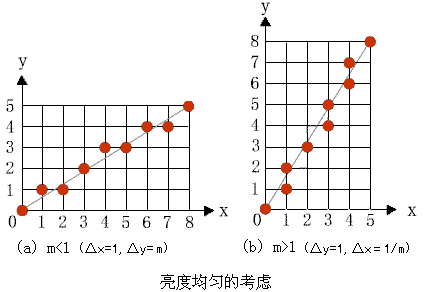
\includegraphics[scale=1]{figure/DDA.png}
	\caption{DDA算法示意图}
	\label{fig:DDA}
\end{figure}

如图\ref{fig:DDA},有如下公式

$$
\begin{cases}
    y_{k+1}=y_k + m \quad \text{$m<=1$}\\
    x_{k+1}=x_k + \frac{1}{m} \quad \text{$m>1$}
\end{cases}
$$
算法的测试如下:在GUI中沿着各种方向画线并观察\\
\begin{figure}[h]
	\centering
	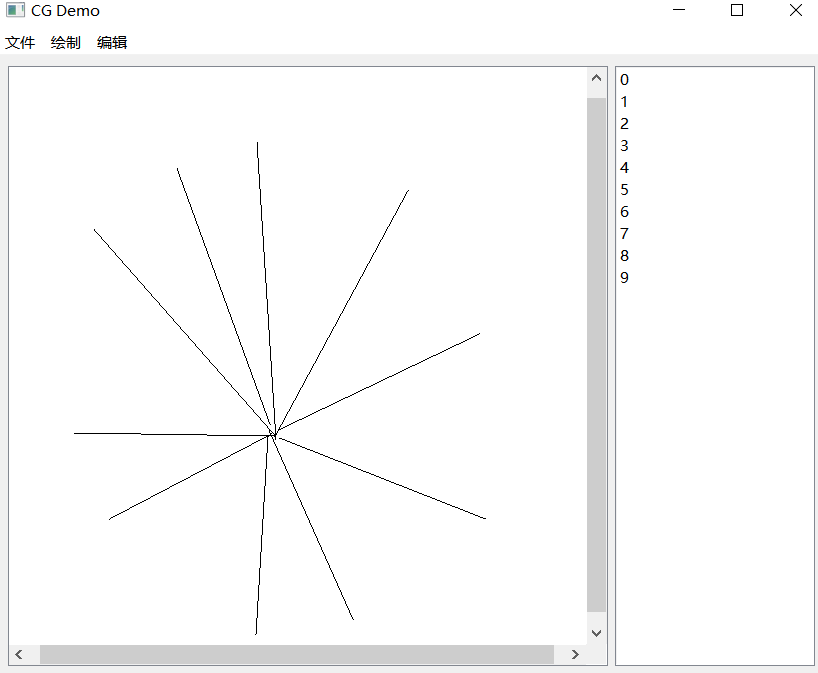
\includegraphics[scale=0.4]{figure/DDA_GUI.png}
	\caption{DDA\_GUI测试示意图}
	\label{fig:DDA_GUI}
\end{figure}

\paragraph{算法评估} 
基于上述的原理对DDA算法性质简单评估
\begin{enumerate}
    \item 优点:DDA算法的计算是增量计算(充分的利用了光栅的特性),每一次计算都是充分的利用了上一次的计算结果,
    所以DDA算法的复杂度小于之前的Naive算法(基于直线方程的)
    \item 缺点:浮点数操作会导致误差的积累,使得结果偏离路线
    \item 缺点:取整和浮点数操作仍然耗时,可以分解增量$\frac{1}{m}$ 和$m$ 为整数和小数,使得计算为整数间的计算而提高效率
\end{enumerate}


\subsubsection{Bresenham}
\paragraph{算法原理}
Bresenham算法\\
Bresenham算法是一种精准而有高效的光栅线段生成算法,他可用于圆和其他曲线显示
的整数增量运算,简单的说就是仍然是选定了一个扫描的方向,然后沿着方向进行扫描,但是
在扫描的过程中对另一个坐标的像素进行选择\\
为了简化像素的选择,Bresenham算法通过引入整形变量去衡量候选像素和实际像素的偏移
并利用对整形变量符号的检测来决定最接近真实路径的像素。\\
\begin{figure}[h]
	\centering
	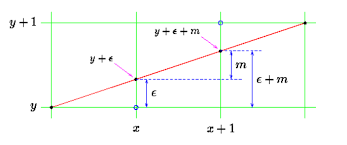
\includegraphics[scale=1]{figure/bresenham.png}
	\caption{Bresenham算法示意图}
	\label{fig:Bresenham}
\end{figure}\\
真实位置$y=mx_{k+1}+b=m(x_k+1)+b$\\
候选像素也就是$y_{k+1}$和$y_k$\\
那么就计算二者的误差(距离差)得到如下的公式
$$
\begin{cases}
    d{1}=y-y_k = m(x_k+1)+b-y_k \\
    d{2}=y_{k+1}-y =y_{k+1}- m(x_k+1)+b
\end{cases}
$$
由于需要比较二者的大小,于是很自然的对二者进行做差
即如下公式\\
\indent $ d{1}-d{2}=2m(x_k+1)-2y_k+2b-1$\\
基于上述的公式得到本算法的核心:决策变量\\
\indent $p_k=\Delta{x}(d_1-d_2)=2\Delta{y}x_k-2\Delta{x}y_k+c$\\
本公式的核心还是在于两个候选像素的误差大小比较(作差)。前面乘上的
$\Delta{x}$主要还是为了优化计算为整数之间的计算而提高效率。
同时$c=2\Delta{y}+\Delta{x}(2b-1)$是一个常量,并会在增量计算中
被忽略
很显然在绘图的时候应该选择误差小的,也就是$p_k$的正负性可以很清楚的
作为像素决策的依据\\\\
目前问题就被转化为如何去计算每一步的$p_k$作选择的依据\\
$p_{k+1}-p_k=2\Delta y x_{k+1}(x_{k+1}-x_k) -2\Delta x( y_{k+1}-y_k)$\\
经过化简之后就可以得到\\
$p_{k+1}=p_k+2\Delta y-2\Delta x( y_{k+1}-y_k)$\\
$$
\begin{cases}
    y_{k+1}-y_k=1 \quad \text{$p_k>0$}\\
    y_{k+1}-y_k=0 \quad \text{$p_k<0$}
\end{cases}
$$
个人的理解就是如\ref{fig:Bresenham}中所示,就是误差的积累
当误差达到一定的大小的时候就只能够去选择下一步的$y_k$,也就是在选择之后需要重新的计算
误差,类似于加法加到一定大小之后取模的操作\\
经过上述的分析之后,很容易就可以得到此算法的工作流程\\
\begin{itemize}
    \item [(1)] 
    计算常量值$\Delta{x}$, $\Delta{y}$, $2\Delta{y}$, $2\Delta{y}-2\Delta{x}$
    \item [(2)]
    循环扫描,对$p_k$的值进行判断
    \item [(3)]
    若$p_k$的值为正,则y加1,同时$p_k=2\Delta{y}-2\Delta{x}$
    \item [(3)]
    反之若$p_k$的值为负,则y不变,同时$p_k=2\Delta{y}$
\end{itemize}

在GUI中测试:\\

\begin{figure}[h]
	\centering
	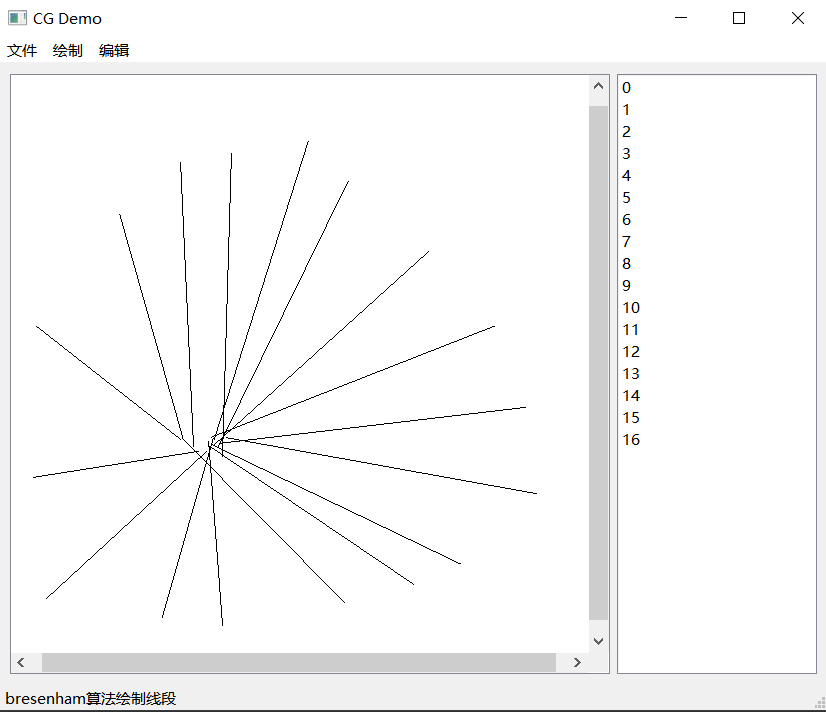
\includegraphics[scale=0.4]{figure/Bre_GUI.png}
	\caption{Bre\_GUI测试示意图}
	\label{fig:Bre_GUI}
\end{figure}

\paragraph{算法评估} 
基于上述的原理对Bresenham算法性质简单评估
\begin{enumerate}
    \item 优点:计算量进一步的减小,每一次的计算都只发生的整数之间,并且都是
    复杂度相对较低的加减法计算,同时只需要判断决策参数的符号,算法效率得到提高
    \item 优点:可以利用并行计算加快图像生成速度
    \item 缺点:稍微复杂,直接看公式可能不能很好的理解
\end{enumerate}

上述的算法大多都经过了在GUI环境下的测试,于是选择在
命令行环境下进行统一测试,分析结果。
整合测试:对上述的三个直线生成代码进行测试,为了方便直接在cli中使用文件测试:\\\\
测试语句如下\\
\indent resetCanvas 600 500\\
\indent setColor 0 0 255\\
\indent drawLine line1 195 363 316 50 Naive\\
\indent setColor 0 255 0\\
\indent drawLine line3 190 343 311 30 DDA\\
\indent setColor 255 0 0\\
\indent drawLine line2 185 323 305 10 bresenham\\
\indent saveCanvas 3\\

测试结果如下\\
\begin{figure}[h]
	\centering
	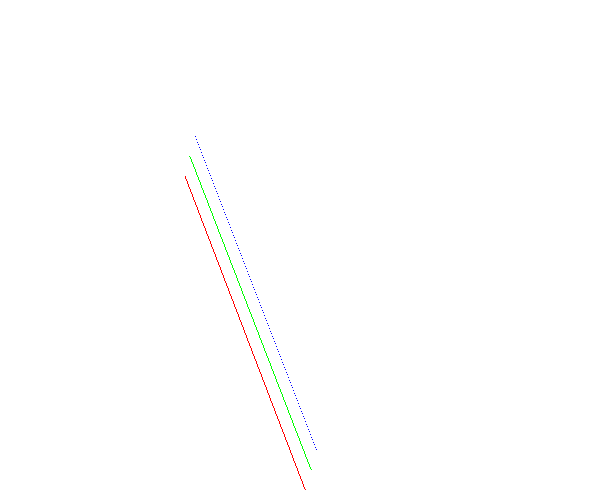
\includegraphics[scale=0.6]{figure/linetest.png}
	\caption{直线绘制算法测试示意图}
	\label{fig:line}
\end{figure}

\subsection{多边形绘制算法}
对于多边形的绘制,本质上就是绘制多条直线,所需要做的就是在顶点之间绘制
直线,进而形成图形的边界。所以本身并不涉及过多的算法实现,只需要在命令行和GUI功能中加上代码,链接
上对应的功能实现就可以\\
分别对Cli和GUI文件进行更改\\

测试输入:\\
\indent resetCanvas 600 500\\
\indent setColor 0 0 255\\
\indent drawPolygon line5 215 353 365 353 365 453 215 453 bresenham\\
\indent drawPolygon line6 235 373 385 373 385 473 235 473 DDA\\
\indent saveCanvas 3\\

测试结果如下\\
\begin{figure}[h]
	\centering
	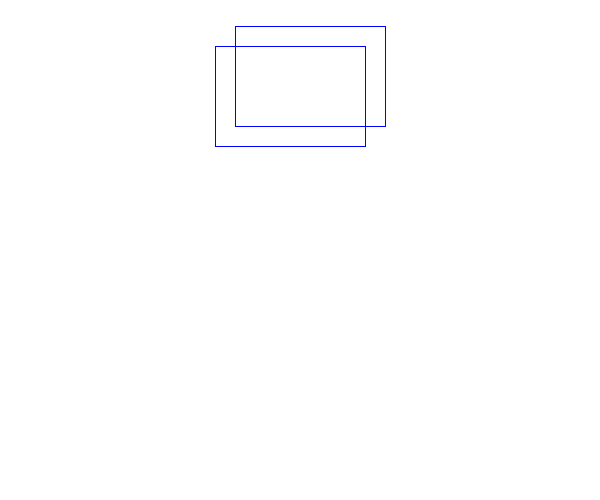
\includegraphics[scale=0.6]{figure/polytest.png}
	\caption{多边形绘制算法测试示意图}
	\label{fig:Poly}
\end{figure}

\subsection{中点圆绘制算法}
\paragraph{算法原理}
中点圆算法\\
首先,椭圆(或者说圆)有若干的性质:
\begin{itemize}
    \item 高度的对称性,也就是只需要生成一部分就可以得到整体
    \item 斜率不断的动态变化,斜率不唯一
\end{itemize}
中点圆算法的原理实际上和Bresenham算法的原理相似,都是通过某一个方向的
扫面,在另一个方向上的候选里去评估错误率,然后进一步的选择哪一个像素点
不同之处就在于所谓的椭圆方程。针对先前已经实现的算法不难发现,这种针对
一个方向扫描的算法的问题就在于用哪个方向,最后的答案往往是根据斜率来决
定,同样的在椭圆这里,由上述的性质知道椭圆绘制需要分段\\
进而计算得到了分段点:\\
\indent $2r_y^2>=2r_x^2y$\\
即这里作为分界分段求解
同时对于段内,需要同样的要引入一个决策变量\\
$p_k=F(x_{k+1},y-\frac{1}{2})=(x_k+1)^2+(y_k-\frac{1}{2})^2-r^2$\\
同理的利用决策变量的符号来决定另一个坐标轴的移动,这个变量表示着候选
像素中点的是否在圆内,也就是标识了所谓的候选点的质量。推导得到了这个决策
变量的增量计算公式如下:\\
区域一:
$$
\begin{cases}
    p_{k+1}=p_k +2r_y^2x_k+3r_y^2 \quad \text{$p<0$}\\
    p_{k+1}=p_k +2r_y^2x_k+3r_y^2-2r_x^2y_k+2r_x^2 \quad \text{$p>=0$}
\end{cases}
$$
区域二:
$$
\begin{cases}
    p_{k+1}=p_k -2r_x^2y_k+3r_x^2 \quad \text{$p<=0$}\\
    p_{k+1}=p_k +2r_y^2x_k+3r_x^2-2r_x^2y_k+2r_y^2 \quad \text{$p>0$}
\end{cases}
$$\\
并根据公式计算决策变量的初始值\\\\
$p_0=r_y^2-r_x^2r_y+\frac{r_x^2}{4}$\\\\
算法的整体流程即如下
\begin{itemize}
    \item [(1)] 
    计算决策变量的初始值,并选择椭圆最上方的点
    \item [(2)]
    沿着X轴循环扫描,根据公式更新决策变量和y值,直到结束区域一
    \item [(3)]
    记忆区域一的最后一个位置,根据公式计算新的决策变量初始值
    \item [(4)]
    沿着Y轴循环扫描,根据对应公式计算决策变量和x值,直到结束区域二
    \item [(5)]
    由先前得到的第一象限的全部图像做图形变化,得到完全椭圆
    \item [(6)]
    根据真实图像所在中心,平移现图像至真实位置结束算法
  \end{itemize}
测试输入:\\
\indent resetCanvas 600 500\\
\indent setColor 0 0 255\\
\indent drawEllipse line7 0 0 200 200\\
\indent drawEllipse line8 100 100 300 300\\
\indent saveCanvas 3\\
测试结果如下(见图\ref{fig:circletest})
\begin{figure}[h]
	\centering
	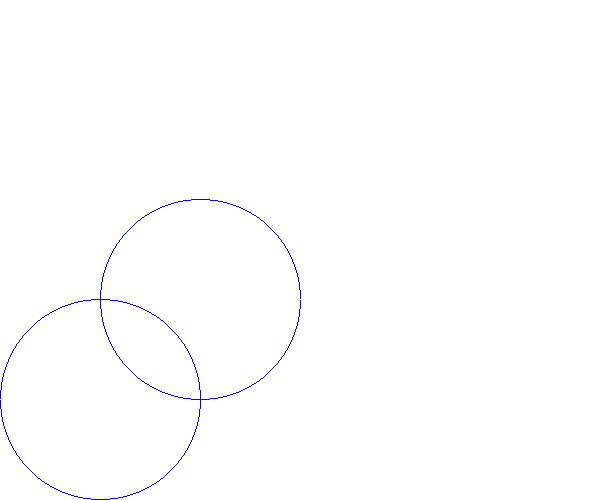
\includegraphics[scale=0.3]{figure/circletest.png}
	\caption{中点圆绘制算法测试示意图}
	\label{fig:circletest}
\end{figure}\\


\subsection{算法正确性检查模块}
\subsubsection{图片读取}
基本步骤如下(详细可见代码:Score\_Test.py)

\begin{itemize}
    \item [(1)] 
    利用os读取到对应图片目录下的所有的文件名字
    \item [(2)]
    拼接得到最终的路径名
    \item [(3)]
    使用PIL库对图片进行读取RGB
    \item [(4)]
    使用Numpy库对数据统一转化为Array
  \end{itemize}

\subsubsection{校验算法}
使用多种方法对多种算法实现的最后结果进行对比和分析\\
(注:仅在本文件为了实现的方便调用了sklearn用于计算余弦相似度。
整个工程的其他位置的代码没有使用任何未经允许的库,如果这也不合规则
也可删除sklearn的调用)
\begin{itemize}
    \item 像素级别对比和差异统计:使用numpy特性扫描图片,
    计算有效区域(即作图区域,可以避免由于作图部分过于稀疏导致的结果差异)
    以及差异区域,计算差异度
    \item 图片整体的相似度计算,利用RGB值对整个图片建模表示,然后计算余
    弦相似度以统计计算图片之间的差异,设置一定的阈值进行警示可能的作图错误
\end{itemize}
如下为一次测试的样例\\

\begin{figure}[h]
	\centering
	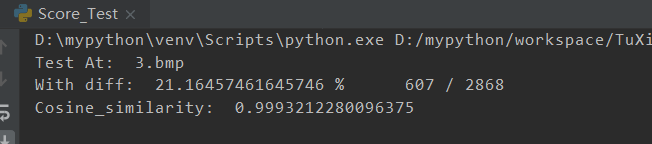
\includegraphics[scale=0.6]{figure/test.png}
	\caption{Score校验算法}
	\label{fig:Score}
\end{figure}
如图\ref{fig:Score},差异度的计算方式为差异度=差异区域像素点数目/着色像素点数目\\
同时计算两个图片向量的余弦相似度作为参考\\
(简单的经验:99.9+\%代表良好,低于99.9\%则可能存在算法绘图错误)\\
\subsection{GUI功能加强}
在GUI方面,为了方便使用加入了使用鼠标直接选中图元的操作
由原框架代码可以知道,选中图元可以通过界面右侧的列表,根据编号选中图元,即选中图元的基本操作
已经被实现,但是由于图元和编号并不显式绑定,所以考虑使用鼠标更加便捷直观的选中图元,对应的就是
需要在鼠标按下和释放的时候,根据当前的状态判断是不是在选中图元的状态。如果是则根据当前的鼠标位置
计算对应选中的图元,然后执行切换选中的过程,后半部分可以通过调用原框架代码的时候达到代码统一化
简洁化的目的\\
基本的实现流程如下

\begin{itemize}
    \item [(1)] 
    利用菜单键进入"Selecting"状态
    \item [(2)]
    在画布界面中点击所需的图元
    \item [(3)]
    鼠标的点击和释放触发信号,并发现当前处于"Selecting"状态,计算得到当前的图元
    \item [(4)]
    如果先前选中图元,则清除先前的选中
    \item [(4)]
    设置当前的选中状态,刷线画布状态,此时后续的处理则会使得图元被红色矩阵包围,显示为选中状态
  \end{itemize}

  \begin{figure}[htbp]
    \centering    %居中
     
    \subfigure[菜单选择] %第一张子图
    {
        \begin{minipage}{7cm}
        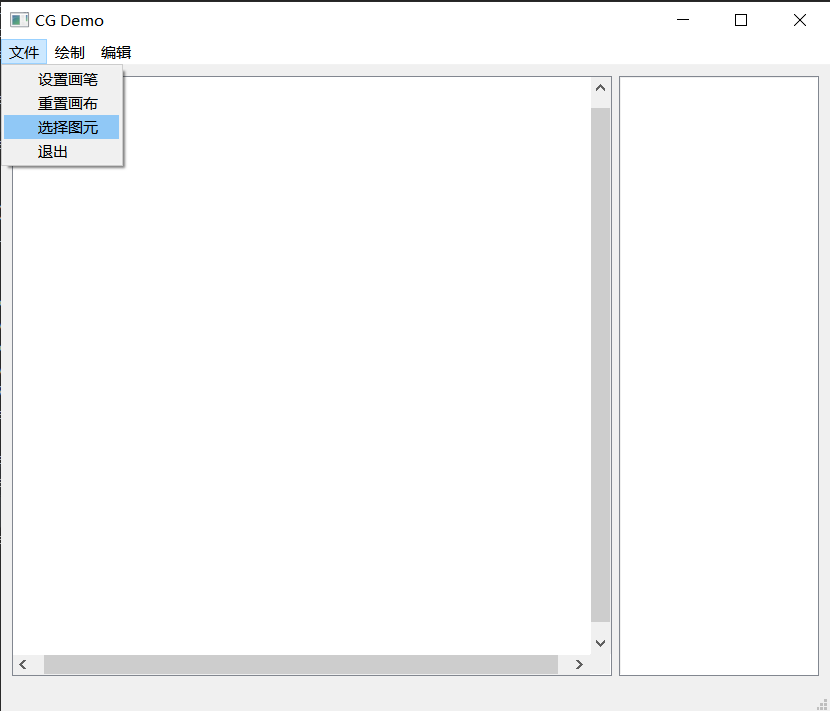
\includegraphics[scale=0.2]{figure/choose.png}   %以pic.jpg的0.5倍大小输出
        \end{minipage}
    }
    \subfigure[鼠标选中] %第二张子图
    {
        \begin{minipage}{7cm}
        \centering      %子图居中
        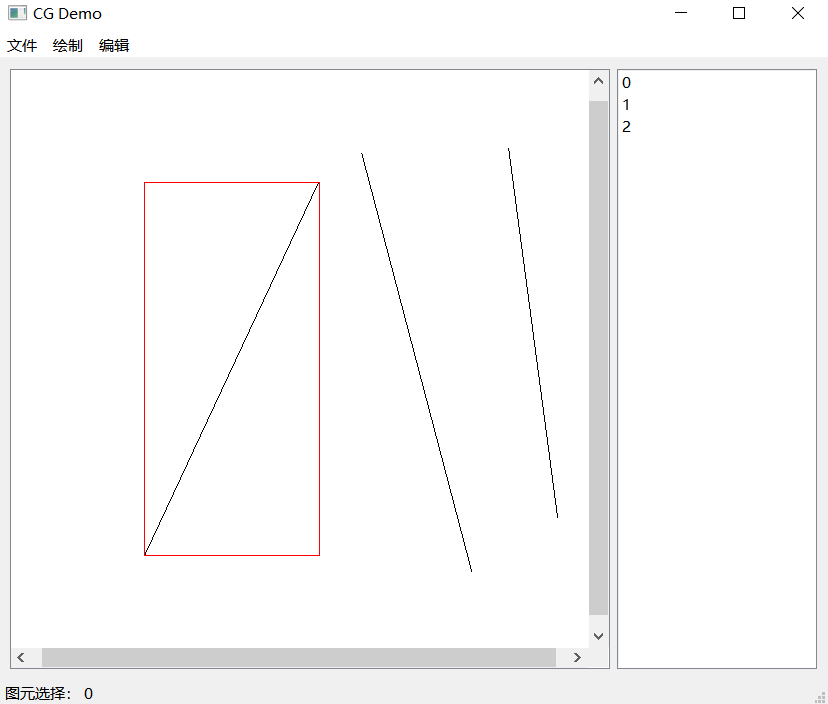
\includegraphics[scale=0.2]{figure/choose2.png}   %以pic.jpg的0.5倍大小输出
        \end{minipage}
    }
     
    \caption{鼠标选中图元测试实例} %  %大图名称
    \label{fig:1}  %图片引用标记
\end{figure}


\section{系统介绍}
目前的CG2020图形学系统已经支持
\begin{itemize}
    \item 命令行和GUI界面调用直线生成算法
    \item 命令行调用多边形生成算法和中点圆生成算法
    \item 在GUI界面中使用鼠标直接的选中所需图元
\end{itemize}

\section{总结}
本次实验基本还是以摸清框架代码结构以及了解QT特性为主,实现的代码量并不大
主要是实现了相对简单明了的直线生成算法以及相对复杂的多边形和中点圆生成算法,同时实现了图片检验模块,为后续的复杂
图像生成的正确性检验做一些准备,最后实现的鼠标选中图元的操作,即是方便操作
同时也是方便于后续复杂图元生成的时候测试和调试工作


\bibliography{xxx}

\begin{thebibliography}{99}  
    \bibitem{ref1}《计算机图形学教程》孙正兴编 
    \bibitem{ref2} \href{https://www.google.com/imghp?hl=zh-CN&ogbl}{Google图片}
\end{thebibliography}

\end{document}

\bibliographystyle{plain}